\section{Experiments}
\label{sec:exp}

% ---- 脉络）--------------------------------------------------------
% 0. Setup：LIBERO 套件；n=500 逐 episode 配对；exact McNemar；预算定义
%    （keep ratio 只作用于 future token，obs token 全保留——务必写清楚）。
% 1. 主结果：成功率--token 预算曲线；对照 native、LoRA 匹配的全上下文、
%    同 router 的 token/tube 删除。对 native 只写"不可区分"。
% 2. 效率：FLOPs、video DiT 延迟、端到端延迟（含固定开销；分别报有无 CUDA graphs）。
%    另含：router + 分配链的开销；LoRA fold 前后的闭环对比与延迟；
%    各预算的 K 档与配额表（Method 4.3 用 \cref{sec:exp} 指向这里）。
% 3. 消融（每个组件一组）：router 训练方式；合并 vs 删除；时间位置 contiguous vs source；
%    空间位置；有无 adapter。
% 4. 泛化：其他套件、LIBERO-Plus、第二个 backbone。
% 5. 分析：router 选择的可视化；激进预算下失败集中的任务。
% 表格放在 tables/ 下，用 \input{tables/<name>} 引入；label 用 tab:<name>。
% ---------------------------------------------------------------------------

\subsection{Experimental Setup}
\label{sec:exp_setup}

We evaluate \method on LIBERO-Spatial, LIBERO-Object and LIBERO-Goal~\cite{liu2023libero}, using the released suite-specific mimic-video checkpoints~\cite{pai2025mimicvideo}.
Each suite contains ten tasks; we run 50 episodes per task and report the success rate over 500 episodes.
Within each suite, all configurations use evaluation seed 0 and the same initial states, allowing outcomes to be paired episode by episode.
The video model runs a single forward pass, and the policy executes five predicted actions before replanning.
Our reference is the native policy: the original video model and action decoder evaluated on the full token sequence.

The budget is the fraction of the 16,800 future tokens retained after the second video DiT block; all 2,400 observation tokens remain.
Keeping 10\%, 20\% and 30\% of the future tokens gives sequences of 4,080, 5,760 and 7,440 tokens, respectively, compared with 19,200 for native.
The spatial allocation keeps 100 of the 300 groups at full resolution at every budget.
In order of increasing priority, the three temporal tiers contain 120, 180 and 300 tubes; their segment counts are $(1,2,4)$, $(3,5,7)$ and $(5,8,10)$ at the three budgets, respectively.

For each suite, we freeze a router trained on that suite and train a fresh rank-16 low-rank adapter (LoRA) in the decoder cross-attention for each budget.
The video model and the original decoder weights remain frozen.
Each adapter is trained for 1,500 steps with the objective in \cref{eq:task_loss}, a learning rate of $4\times10^{-5}$, 100 warmup steps, cosine decay and an effective batch size of eight.
The Object router uses a different initialization and training recipe: fixed segment counts of $8/6/4$ and pure distillation, whereas the Spatial and Goal routers use $12/10/8$ and the additional ground-truth term of weight 0.02.
This difference concerns router training; the budget-specific adapters use the same objective on all three suites.
We use one training seed per configuration.

We compare paired success outcomes with two-sided exact McNemar tests and apply Holm correction over the nine suite--budget comparisons with native, at a significance level of 0.05.
The error bars and native bands in \cref{fig:main_results} are Wilson 95\% confidence intervals for the individual success rates.
Non-significant comparisons are described as statistically indistinguishable at this sample size.

\subsection{Main Results}
\label{sec:exp_main}

\begin{figure*}[t]
  \centering
  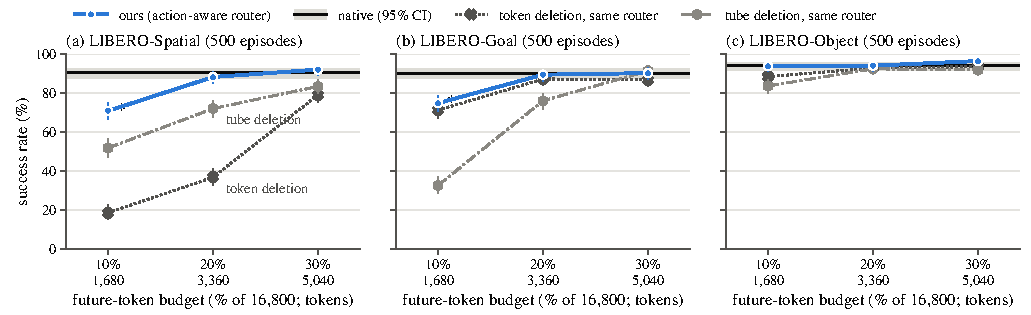
\includegraphics[width=\linewidth]{fig4_main_results.pdf}
  \caption{\textbf{Success rate versus future-token budget.}
  Each point uses 500 paired episodes; the 2,400 observation tokens are always kept.
  Blue: \method; black line and grey band: native, which reads all 16,800 future tokens.
  Grey curves (Spatial only): token or tube deletion using the same router and the same budgets, each with its own trained low-rank adapter.
  Token deletion keeps the highest-scoring future tokens; tube deletion keeps the highest-scoring tubes with all 14 frames.
  Error bars and band: Wilson 95\% confidence intervals.
  Asterisks mark \method results that differ from native under two-sided exact McNemar tests with Holm correction over the nine suite--budget comparisons.
  The Object router uses the distinct training recipe described in \cref{sec:exp_setup}.}
  \label{fig:main_results}
\end{figure*}

At 20\% of the future tokens, \method is statistically indistinguishable from native on all three suites (\cref{fig:main_results}).
Success rates are 88.2\% on Spatial, 94.0\% on Object and 89.4\% on Goal, compared with 90.4\%, 94.0\% and 90.2\% for native.
The corresponding uncorrected paired-test $p$-values are 0.22, 1.00 and 0.71; none is significant after correction.
At this operating point, the remaining video blocks and action decoder receive 5,760 tokens, or 30\% of the native sequence.

The effect of a tighter budget differs across suites.
At 10\% of the future tokens, success falls to 70.8\% on Spatial and 74.8\% on Goal, both significantly below native after correction, while Object reaches 93.8\% and remains statistically indistinguishable from native.
At 30\%, the respective success rates on Spatial, Object and Goal are 92.0\%, 96.4\% and 90.2\%; all three are statistically indistinguishable from native after correction.
Thus, 20\% of the future tokens is the smallest tested budget at which all three suites are statistically indistinguishable from native in this evaluation.

\TODO{Remaining experiments: merging versus deletion; contiguous versus source temporal positions; E1--E3 action-relevance analyses; transfer to DiT4DiT if included.}
\TODO{Efficiency: FLOPs and latency of the deployed contiguous-t budgets have not been measured.}
